\documentclass[letter]{ieicej}
\usepackage[dvipdfmx]{graphicx,xcolor}
\usepackage[fleqn]{amsmath}
\usepackage{newtxtext}
\usepackage[varg]{newtxmath}
\usepackage{url}
\typeofletter{研究速報}
\field{}
\jtitle{LLMエージェントの閾値型要約における再帰置換と差分保持の比較}
\etitle{Comparing Recursive Replacement and Delta Retention under Threshold-Triggered Summarization for LLM Agents}
\authorlist{\authorentry{著者未設定}{Author details pending}{}{}\MembershipNumber{}}
\jalcdoi{???????????}
\begin{document}
\maketitle
\begin{abstract}
LLMエージェントの同一閾値下で再帰置換と差分保持を既知4課題で比較した．成功は3件から2件へ減り，差分が届いた共通成功課題も増費用となった．使用量不明1呼出しを残し，品質を保つ総費用削減は確認できなかった．
\end{abstract}
\begin{keyword}
LLMエージェント，文脈圧縮，差分要約，閾値制御，費用評価
\end{keyword}
\begin{eabstract}
With a common threshold, we compare recursive replacement with an immutable-summary, object-delta bundle on four known tasks. Success falls from three to two tasks. One call has unknown usage; an activated common-success task costs more. The experiment does not establish quality-preserving whole-job savings.
\end{eabstract}
\begin{ekeyword}
LLM agents, context compression, delta summarization, threshold control, cost evaluation
\end{ekeyword}


\section{まえがき}
大規模言語モデル（LLM）によるエージェントは，推論と行動を繰り返し\cite{yao2023react}，生成したコードで外部環境を操作する\cite{wang2024codeact}．長い課題では，蓄積した行動と観測を後続の入力に繰り返し含める費用が増える．履歴要約はこの入力を短くするが，要約の作成自体にも入力・出力費用がかかる．更に，課題の途中で必要な情報を失うと，再取得や誤った操作につながり得る．

本稿では，要約を再び要約するときの保持表現に着目する．旧要約と新しい履歴をまとめ直す再帰置換は，重複や古い記述を整理できる一方，既に記録した状態もモデルが書き直す．旧要約を固定して新情報を追加すれば，旧要約全体の再出力を要求せずに済むが，古い状態や冗長な記述が後続入力に残る．このトレードオフが，課題の最終成功と要約費を含む総費用にどう現れるかを調べる．

プロンプト圧縮\cite{jiang2024longllmlingua}，長期エージェントの圧縮方針の最適化\cite{kang2026acon}，キャッシュを考慮した文脈管理\cite{xu2026tokenpilot}を踏まえ，本比較では通常の入力長閾値と実行予算を共通にし，第2要約の処置を変える．比較対象は，再帰置換と，\emph{旧要約保持・明示的な差分object出力・ホストによる結合}の組である．既知4課題の全実行を対象に，成功を失わずに全呼出しの論理入出力を減らせるかを評価する．結果は成功喪失と使用量不明を含み，この目標の達成を支持しなかった．

\section{共通閾値下の保持表現}
\subsection{ハーネスと比較方式}
図\ref{fig:architecture}に構成を示す．actorは課題実行，focusは履歴要約を担当するLLM呼出しであり，同じモデルを用いる．ホストは完全な履歴を保存し，actorにはシステム指示，課題，採用済み要約，要約位置より後の履歴を提示する．直近2ターンは要約対象から除外する．

\begin{figure*}[t]
\centering
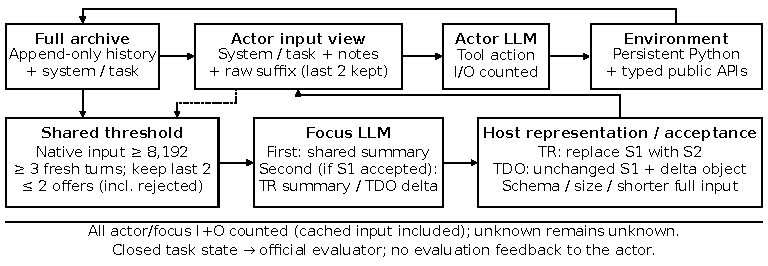
\includegraphics[width=130mm]{figures/architecture_p143.pdf}
\caption{共通の入力長閾値で保持表現を比較するハーネス．}
\ecaption{Harness comparing retained representations under a common input-length threshold.}
\label{fig:architecture}
\end{figure*}

TR（threshold recursive）は通常の再帰要約，TDO（threshold delta object）は旧要約を保持する差分要約である．両方式ともactor入力が8,192トークン以上，前回機会以後の新規完了ターンが3以上で要約機会を設ける．機会は未送信・不採用を含めて最大2回とする．初回の入力構成と出力契約は共通であり，第1要約を採用できた場合だけ，第2機会の処置を分ける．

旧要約を$S_1$，新たな対象履歴を$H_2$とする．両方式とも$S_1$と$H_2$をfocusへ提示する．TRはこれらをまとめた要約$S_2$を返す．TDOは$S_1$を参照しながら，新情報を記述した単一の差分object $D_2$だけを返す．ホストが採用した後の要約部分は，
\begin{equation}
 \text{TR}: S_2,\qquad \text{TDO}: (S_1,D_2)
 \label{eq:representation}
\end{equation}
となる．TDOの$S_1$は保存済み文字列をそのまま用い，モデルに旧要約の再出力を要求しない．初回が不採用なら両方式とも通常の要約経路を用いる．

\subsection{共通の採用制約}
要約objectは完了事項，利用可能状態，残作業，不確実性の4フィールドを持つ．保存する要約の合計は8,192文字，各フィールド合計32項目，1項目2,048文字以下とする．TDOでは$S_1$と$D_2$の合計に上限を適用する．構造検査の後，次のactor入力全体をnative tokenizerで計数し，従来の表示より短い場合だけ採用する．指示・課題・tools・予算通知・残存履歴を含めた判定であり，差分だけが短ければよいわけではない．共有の残予算と文脈長も確認する．

不採用または未送信では旧表示を維持する．既知の使用量は不採用focusも計上し，使用量が不明になればその条件を停止する．入力帰属のための追加計数\cite{singh2026tca}は両方式に共通で，その時間も作業上限に含む．

\section{実験方法}
\subsection{課題と実行条件}
AppWorld\cite{trivedi2024appworld}の既知4課題（写真操作，精算，返金，CSV処理）に対し，TRとTDOを各1回，計8条件実行した．model seedの基点は157，world seedは42とし，役割ごとの呼出し数でmodel seedを増分する．課題を上記の順とし，奇数課題ではTRから，偶数課題ではTDOから実行する．各条件で新しい課題状態を用意し，両方式の初回入力が一致することを検査する．

先行する同じ4課題・seedの16,384閾値比較では，両方式が3/4成功，費用572,405トークンで同値となり，第2差分処置は全課題で未発動だった．そこで本比較では，発動範囲を調べるため共通閾値8,192を結果観測後に選定した．作業上限も1,800秒から1,200秒へ変更するため，先行比較との費用差を閾値だけの効果とは扱わず，今回の同条件TR/TDO対を評価する．

actorとfocusにはMiniMax-M3（GGUF，IQ4\_XS）を用いる．llama.cpp b11669，文脈長65,536，KV cache q8\_0，並列数1，温度はactor 1.0，focus 0.7とする．計算機はApple M3 Ultra，メモリ256 GiBである．各条件の上限は全モデル要求80回，論理入出力450,000トークン，作業1,200秒，1回の通常出力4,096トークンとする．環境APIは写真操作160要求，他の課題80要求を上限とする．セットアップ，後片付け，評価には別に有限の上限を設ける．実装と全条件を公開する\footnote{\url{https://github.com/sophiria1225/AI-}}．

\subsection{費用と品質}
費用は，条件$p$のactorとfocusを含む全呼出し集合$\mathcal{C}_p$について，実入力$I_c$と実出力$O_c$を足した
\begin{equation}
 T_p=\sum_{c\in\mathcal{C}_p}(I_c+O_c)
 \label{eq:cost}
\end{equation}
とする．cached inputを控除せず，失敗時や不採用要約の既知費用も含める．したがって，キャッシュを考慮した金銭費用とは区別する\cite{xu2026tokenpilot}．要約役を含む費用評価はACON\cite{kang2026acon}にもあり，本稿では保持表現の評価指標として用いる．使用量不明があれば既知小計と不明件数を示し，確定総費用や削減率は算出しない．

最終品質は，実行後の状態に対する公式評価器の成否で測る．評価の詳細は実行中のモデルへ返さない．課題$t$の成功を$y_{t,p}\in\{0,1\}$とし，TRの成功をTDOが失った課題数を
\begin{equation}
 L=\sum_{t=1}^{4}\mathbf{1}[y_{t,\mathrm{TR}}=1,\ y_{t,\mathrm{TDO}}=0]
 \label{eq:loss}
\end{equation}
とする．成功数の総計だけでなく，課題ごとの保持を確認する．費用は全4対と，両方式が成功した課題集合$\mathcal{S}$の双方で比較する．未評価を失敗へ，使用量不明を0へ置き換えない．

固定した効用条件は，全8条件の評価・会計が揃い，$L=0$，$\mathcal{S}$が空でなく，全4対と共通成功対の両方でTDOの費用が小さいことである．処置への到達は，第2object focusの既知送信と，その差分を含むactor入力で確認する．処置前の履歴の対応も検査し，介入を伴う開発判定と集計上の効用条件を分けて報告する．

\section{結果と考察}
\subsection{課題別の成否と費用}
表\ref{tab:p143-cells}と図\ref{fig:p143-cost}に全8条件を示す．
\begin{table*}[t]
\caption{課題別の成否と論理入出力．不明呼出しは0補完しない．差分付きactorは既知使用量の呼出し数．}
\ecaption{Task outcomes and logical input/output. Known subtotals are distinguished from unknown usage.}
\label{tab:p143-cells}
\centering
\begin{tabular}{llrrrl}
\hline
課題 & 方式 & 最終成否 & 既知token小計 & 不明呼出し & 差分付きactor \\ \hline
写真操作 & TR & 成功 & 200,016 & 0 & 0\\
写真操作 & TDO & 失敗 & 149,194 & 1 & 0\\
精算 & TR & 成功 & 182,483 & 0 & 0\\
精算 & TDO & 成功 & 218,061 & 0 & 13\\
返金 & TR & 成功 & 68,923 & 0 & 0\\
返金 & TDO & 成功 & 68,923 & 0 & 0\\
CSV処理 & TR & 失敗 & 194,187 & 0 & 0\\
CSV処理 & TDO & 失敗 & 110,147 & 0 & 6\\
\hline
\end{tabular}
\end{table*}
\begin{figure*}[t]
\centering
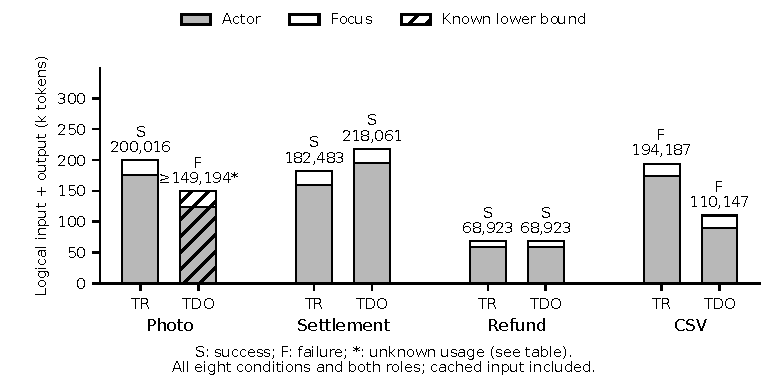
\includegraphics[width=130mm]{figures/p143_cost.pdf}
\caption{全8条件のactor・focus別論理入出力と最終成否．斜線は確定総費用ではない既知小計を示す．}
\ecaption{Logical input/output by role and final outcomes. Hatched bars denote known lower bounds.}
\label{fig:p143-cost}
\end{figure*}
\subsection{品質と全費用の比較}
全8条件を評価し，成功はTRが3/4，TDOが2/4だった．写真操作でTRの成功をTDOが失い，$L=1$となった．TDOの同課題はモデル呼出し中の時間上限で停止し，actor 1呼出しの使用量が不明だった．既知小計はTRが645,609，TDOが546,325トークンであるが，この差を総費用削減とは扱わない．固定した全8条件の会計充足条件を満たさないため，全体と共通成功集合の確定費用差・削減率はいずれも算出せず，効用条件と開発条件は不成立だった．

共通成功は精算と返金の2課題である．個別の確定値を見ると，精算はTDOが35,578トークン多く，返金は同値だった．CSV処理ではTDOが84,040トークン少なかったが，両方式ともAPI上限で停止し失敗した．この減少は，成功を保った節約の事例ではない．

\subsection{差分処置の作動範囲}
TDOの第2object focusは写真操作，精算，CSV処理の3課題で既知の送信を確認した．差分が採用されてactor入力に届いたのは精算とCSV処理の2/4課題で，差分付きの既知actor呼出しはそれぞれ13回，6回だった．返金では第2差分処置が作動しておらず，その成功を差分保持の効果例には数えない．写真操作でも差分付きactorは0回であり，旧要約保持が成功喪失の原因だとまでは特定できない．

差分が届いた唯一の共通成功課題である精算では，focus費用は52トークン減った一方，actor費用は35,630トークン増えた．旧要約の再出力を要求しない処置が，後続入力や行動を含む総費用の減少に直結しない実例である．ただし，増分を旧要約の保持量だけに帰属する比較ではなく，処置後の履歴と呼出し数の変化を含む．以上より，本条件では機構の作動は観測できたが，品質を保つ全仕事費用削減は確認できなかった．


本比較は既知4課題，単一モデル・量子化・seedと結果観測後に選んだ閾値による開発評価である．seedは過去の別比較でも用いており，未見課題への独立確認ではない．結果は保持・出力指示・ホスト結合を合わせた処置の比較であり，各要素の単独効果を分離しない．同じ閾値でも処置後の履歴，呼出し回数，実時間は変わるため，課題ごとの成否と全呼出しの費用から解釈する．

\section{むすび}
共通の入力長閾値で，再帰置換と旧要約保持・object差分・ホスト結合を比較した．差分は2課題のactor入力に届いたが，成功は3/4から2/4へ減った．差分が届いた共通成功課題では総費用も増えた．使用量不明1呼出しを残すため全体の削減率は確定せず，品質を保つ全仕事費用削減は確認できなかった．旧要約の再出力を省く局所的な処置は，その後の課題実行を含む効用を保証しない．

% Verified official publication metadata; all authors retained.
% Bibliographic source URLs and detailed verification are in references.bib
% and the private claim-source mapping. Only TCA below is a preprint.
\begin{thebibliography}{9}
\bibitem{yao2023react}
S. Yao, J. Zhao, D. Yu, N. Du, I. Shafran, K. Narasimhan, and Y. Cao,
``ReAct: Synergizing reasoning and acting in language models,''
Proc. ICLR, May 2023.

\bibitem{wang2024codeact}
X. Wang, Y. Chen, L. Yuan, Y. Zhang, Y. Li, H. Peng, and H. Ji,
``Executable code actions elicit better LLM agents,''
Proc. ICML, PMLR, vol.235, pp.50208--50232, July 2024.

\bibitem{jiang2024longllmlingua}
H. Jiang, Q. Wu, X. Luo, D. Li, C.-Y. Lin, Y. Yang, and L. Qiu,
``LongLLMLingua: Accelerating and enhancing LLMs in long context scenarios via prompt compression,''
Proc. ACL, vol.1, pp.1658--1677, Aug. 2024.
doi: 10.18653/v1/2024.acl-long.91.

\bibitem{kang2026acon}
M. Kang, W.-N. Chen, D. Han, H. A. Inan, L. Wutschitz, Y. Chen,
R. Sim, and S. Rajmohan,
``ACON: Optimizing context compression for long-horizon LLM agents,''
Proc. ICML, PMLR, vol.306, pp.55321--55375, July 2026.

\bibitem{xu2026tokenpilot}
B. Xu, Z. Xue, D. Chen, C. Fu, C. Wu, C. Huang, C. Jiang, J. Fang,
X. Deng, Y. Chen, Y. Yao, X. Wang, J. Shang, H. Chen, and N. Zhang,
``TokenPilot: Cache-efficient context management for LLM agents,''
Findings of ACL: EMNLP 2026, pp.19034--19049, Oct. 2026.

\bibitem{singh2026tca}
V. K. Singh, P. Priyam, and G. Bhowmick,
``Total cost of agency: Exact attribution of memory injection cost in multi-agent LLM workflows,''
arXiv preprint arXiv:2609.23790v1, Sept. 2026.
\bibitem{trivedi2024appworld}
H. Trivedi, T. Khot, M. Hartmann, R. Manku, V. Dong, E. Li, S. Gupta,
A. Sabharwal, and N. Balasubramanian,
``AppWorld: A controllable world of apps and people for benchmarking interactive coding agents,''
Proc. ACL, vol.1, pp.16022--16076, Aug. 2024.
doi: 10.18653/v1/2024.acl-long.850.

\end{thebibliography}

\end{document}
